\documentclass[hyperref={pdfpagelabels=false}]{beamer}
\usepackage{lmodern}
\usetheme{Frankfurt}
\usecolortheme{crane}
\usepackage[noend]{algorithmic}
\usepackage{tikz}
\usepackage{wrapfig}
\usepackage{lipsum}
\usepackage{sidecap}
\usepackage{graphicx}
\usepackage{subcaption}
\usepackage{float}
\usepackage{amsmath}
\usepackage{hyperref}
\hypersetup{
	colorlinks=true,
	linkcolor=blue,
	filecolor=magenta,
	urlcolor=cyan,
}
% \usepackage{enumitem}
\usetikzlibrary{shapes,arrows,positioning,calc}
\usetikzlibrary{decorations.pathreplacing}
% below code is used for making diagrams in slides
% do not delete it
\tikzset{
	block/.style = {
		draw,
		fill=white,
		rectangle,
		minimum height=1.8em,
		minimum width = 10em
	},
	block2/.style = {
		draw,
		fill=white,
		rectangle,
		minimum height=3.7em,
		minimum width=6em
	},
	sum/.style = {
		draw,
		fill=white,
		circle,
		inner sep=0pt,
		minimum size = 0.5cm
	},
	pinstyle/.style = {
		pin edge={to-,thin,black}
	}
}

\title{PRESENT Cipher}  
\author{\texttt{Walkie Talkie}} 
\institute{
	
\includegraphics[scale=0.08]{logoiitbh}
	
	Department of \texttt{EECS}\\ 
	Indian Institute of Technology Bhilai}

\begin{document}
	\begin{frame}
	\titlepage

\end{frame} 

\AtBeginSection[]
{
	\begin{frame}<beamer>
	\frametitle{Outline}
	\tableofcontents[currentsection]
\end{frame}
}

\section{Introduction}


\begin{frame}{The Present Cipher}
\begin{itemize}
    \item Ultra-Lightweight block cipher.
    \item Developed by the Orange Labs (France), Ruhr University Bochum (Germany) and the Technical University of Denmark in 2007.
    \item Supports 64 bits block size and 80 or 128 bits key sizes with 31 rounds.
    \item Designed to be used in micro-controllers and hardware where high chip performance and low power consumption are required.
\end{itemize}
\end{frame}

\begin{frame}{Substitution/ Permutation}
\begin{figure}[H]
    \centering
    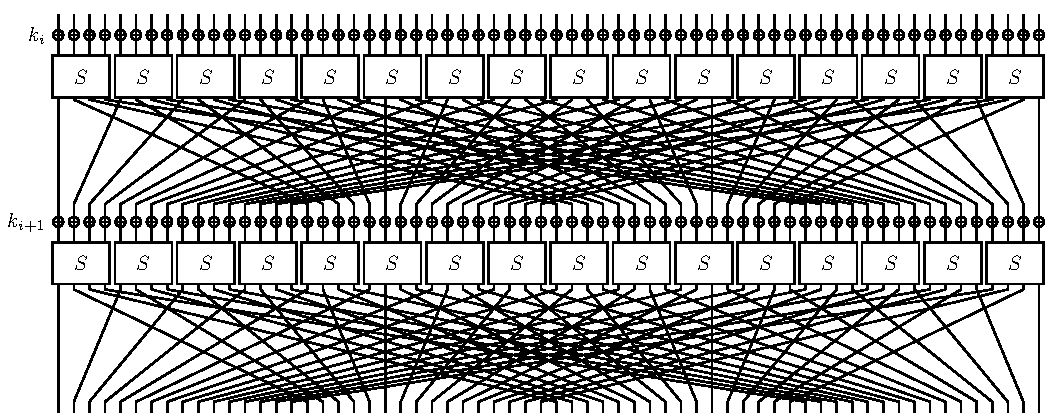
\includegraphics[width=\linewidth]{PRESENT_diagram.pdf}
\end{figure}
\begin{center}
    \scalebox{0.95}{
    \begin{tabular}{ |c||c|c|c|c|c|c|c|c|c|c|c|c|c|c|c|c| }
        \hline
        $x$ & 0 & 1 & 2 & 3&4& 5& 6&7&8&9&A&B&C&D&E&F  \\ \hline
        $S[x]$& C & 5 & 6& B &9 &0 &A &D& 3& E &F& 8& 4 &7& 1& 2 \\ \hline
    \end{tabular}}\\
    % Image source : iacr.org/authors/tikz/
\end{center}
\end{frame}

\section{Cipher Specifications}

\begin{frame}[c]{Cipher Design}
\begin{itemize}
    \item PRESENT-80 is an example of SP-network.
    \item 4-bit S-Box is applied 16 times in parallel for the 64-bit input during each round.
    \begin{block}{High level psuedo-code of PRESENT algorithm}
        \begin{algorithmic}[1]
        \STATE{generateRoundKeys()}
        \FOR{$i=1$ \TO $31$ }
            \STATE {addRoundKey(\textsc{State},$K_i$)}
            \STATE {sBoxLayer(\textsc{State})}
            \STATE {pLayer(\textsc{State})}
        \ENDFOR
        \STATE addRoundKey(\textsc{State},$K_{32}$)
        \end{algorithmic}
    \end{block}
\end{itemize}
\end{frame}

\begin{frame}{Cipher Design contd.}
       \begin{block}{Add Round Key}
           \begin{itemize}
               \item Round key $K_i = k_{63},k_{62} \dots k_0$ for $1\leq i \leq 32$.
               \item Current state $S = s_{63},s_{62}\dots s_0$.
               \begin{eqnarray*}
                    S \xrightarrow{} S \oplus K_i \\
                    \implies s_t \xrightarrow[]{} s_t \oplus k_t
                \end{eqnarray*}
                for $0\leq t\leq 63$
           \end{itemize}
       \end{block}
\end{frame}

\begin{frame}{Substitution Layer}
     PRESENT S-Box satisfies the following conditions.
    \begin{itemize}
        \item For any fixed input difference $\Delta_I \in \mathbb{F}_2^4,\Delta_I \not = 0$ and output difference $\Delta_O \in \mathbb{F}_2^4,\Delta_I \not = 0$, the following condition is satisfied
        \begin{equation*}
            |\{ x \in \mathbb{F}_2^4~~ \vert~~ S(\Delta_I +x) + S(x) = \Delta_O \}| \leq 4
        \end{equation*}
        \item For any fixed input difference $\Delta_I \in \mathbb{F}_2^4,\Delta_I \not = 0$ and output difference $\Delta_O \in \mathbb{F}_2^4$ such that $wt(\Delta_O) = wt(\Delta_I) = 1$, the following condition is satisfied
        \begin{equation*}
            \{ x \in \mathbb{F}_2^4~~ \vert~~  S(\Delta_I +x) + S(x) = \Delta_O  \} = \Phi
        \end{equation*}
        where $wt(x)$ is the hamming weight of $x$.
    \end{itemize}
\end{frame}

\begin{frame}{Cipher Design Contd.}
    \begin{block}{Permutation Layer}
        \begin{itemize}
            \item Bit permutation.
            \item Bit $i$ of \textsc{STATE} is moved to bit position $P(i)$.
        \end{itemize}
        \begin{eqnarray*}
         P(i) =  \begin{cases}
              16.i~~ mod~~ 63 & i \in \{0,1,\dots 62 \}\\
              63 & i = 63
           \end{cases}
        \end{eqnarray*}
    \end{block}
\end{frame}


\begin{frame}{Key schedule Algorithm}
We discuss the 80-bit key schedule algorithm.
 \begin{figure}[H]
	\centering
	\minipage{\textwidth}
	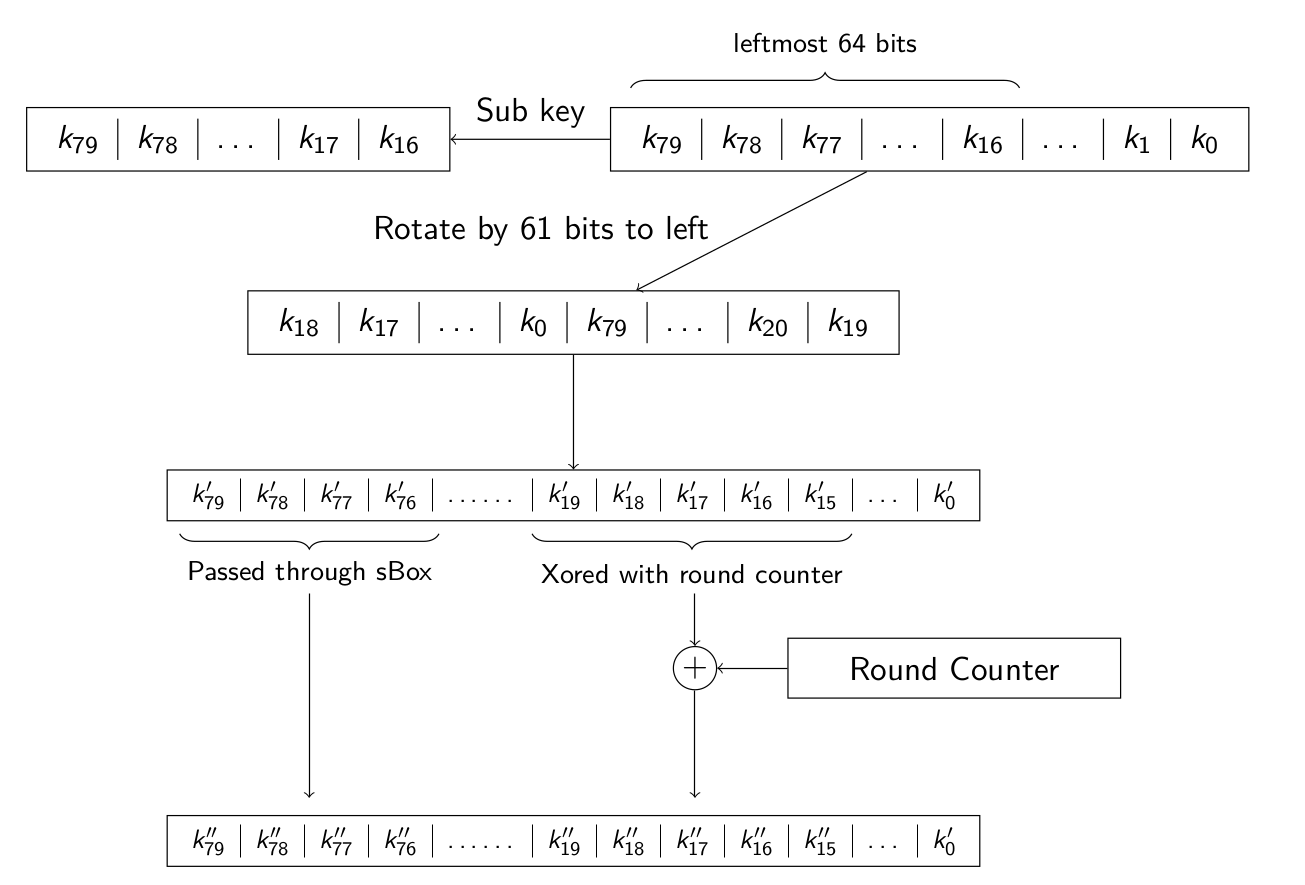
\includegraphics[width=\linewidth]{key.png}
	\endminipage
	\caption{Key schedule}
	\label{fig:key}
\end{figure}
\end{frame}

\section{DC}

\begin{frame}{Round Reduced Attack}
\begin{figure}[H]
        \centering
        \minipage{\textwidth}
        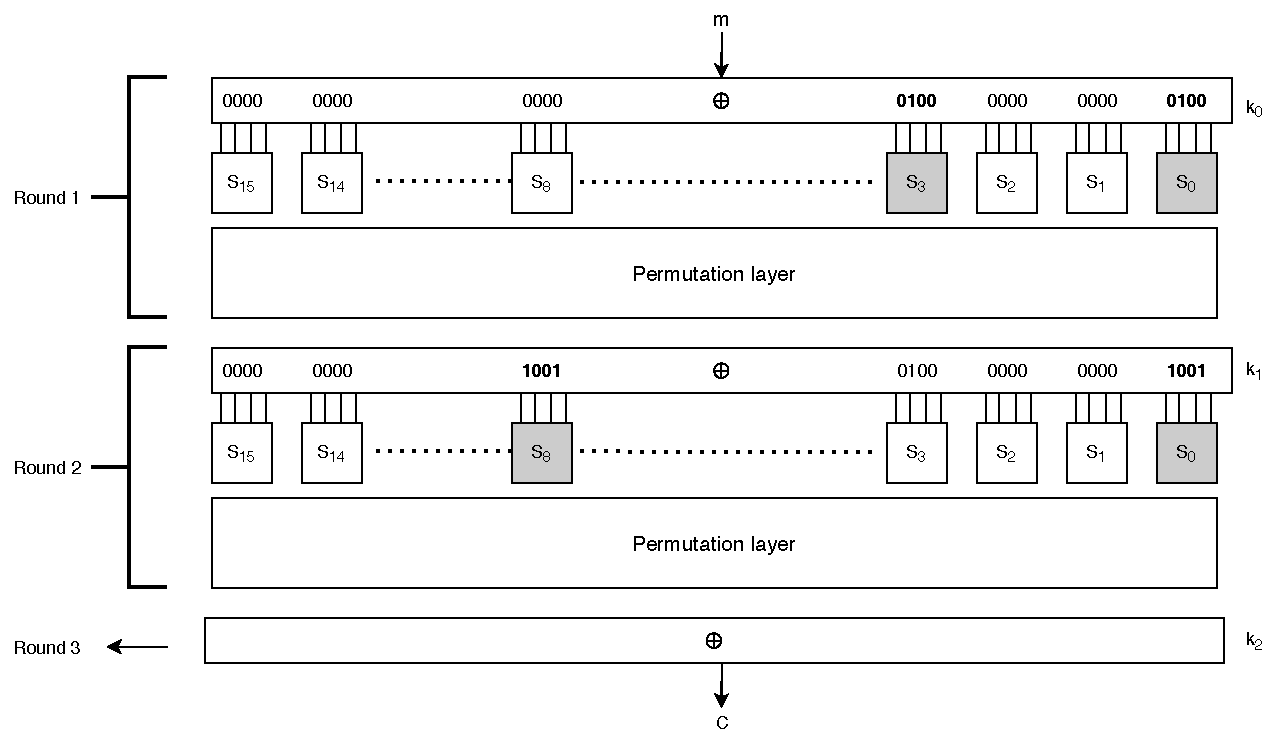
\includegraphics[width=\linewidth]{DC1.pdf}
        \endminipage
        \caption{Attack Model}
    \end{figure}
\end{frame}

\begin{frame}{The Difference Distribution Table}
\begin{figure}[h!]
    \caption{DDT of the S-box}
    \centering
    \scalebox{0.8}{
    \begin{tabular}{ |c||c|c|c|c|c|c|c|c|c|c|c|c|c|c|c|c| }
        \hline
         & 0 & 1 & 2 & 3&4& 5& 6&7&8&9&A&B&C&D&E&F  \\ \hline \hline
         0& 16 & 0 & 0 & 0 &0 &0 &0 &0& 0& 0 &0& 0& 0 &0& 0& 0 \\ 
         1& 0 & 0 & 0 & 4 & 0 & 0 & 0 & 4 & 0 & 4 &0& 0& 0 &4& 0& 0 \\
         2& 0 & 0 & 0 & 2 & 0 & 4 & 2 & 0 & 0 & 0 &2& 0& 2 &2& 2& 0 \\
         3& 0 & 2 & 0 & 2 & 2 & 0 & 4 & 2 & 0 & 0 &2& 2& 0 &0& 0& 0 \\
         4& 0 & 0 & 0 & 0 & 0 & 4 & 2 & 2 & 0 & 2 &2& 0& 2 &0& 2& 0 \\
         5& 0 & 2 & 0 & 0 & 2 & 0 & 0 & 0 & 0 & 2 &2& 2& 4 &2& 0& 0 \\
         6& 0 & 0 & 2 & 0 & 0 & 0 & 2 & 0 & 2 & 0 &0& 4& 2 &0& 0& 4 \\
         7& 0 & 4 & 2 & 0 & 0 & 0 & 2 & 0 & 2 & 0 & 0 & 0 & 2 & 0 & 0 & 4\\
         8& 0 & 0 & 0 & 2 & 0 & 0 & 0 & 2 & 0 & 2 & 0 & 4 & 0 & 2 & 0 & 4\\
         9& 0 & 0 & 2 & 0 & 4 & 0 & 2 & 0 & 2 & 0 & 0 & 0 & 2 & 0 & 4 & 0\\
         A& 0 & 0 & 2 & 2 & 0 & 4 & 0 & 0 & 2 & 0 & 2 & 0 & 0 & 2 & 2 & 0\\
         B& 0 & 2 & 0 & 0 & 2 & 0 & 0 & 0 & 4 & 2 & 2 & 2 & 0 & 2 & 0 & 0\\
         C& 0 & 0 & 2 & 0 & 0 & 4 & 0 & 2 & 2 & 2 & 2 & 0 & 0 & 0 & 2 & 0\\
         D& 0 & 2 & 4 & 2 & 2 & 0 & 0 & 2 & 0 & 0 & 2 & 2 & 0 & 0 & 0 & 0\\
         E& 0 & 0 & 2 & 2 & 0 & 0 & 2 & 2 & 2 & 2 & 0 & 0 & 2 & 2 & 0 & 0\\
         F& 0 & 4 & 0 & 0 & 4 & 0 & 0 & 0 & 0 & 0 & 0 & 0 & 0 & 0 & 4 & 4\\ \hline
    \end{tabular}
    }
\end{figure}
\end{frame}

\begin{frame}{Differential Characteristics}
\begin{table}[h!]
	\caption{Characteristics}
	\centering
	\begin{tabular}{ |c||c|c|c| }
		\hline
		Rounds & & Diff. & Prob. \\ \hline \hline
		I& & $x_0 = 4$, $x_4 = 4$ &  \\ 
		$R_1$& $k_0$ & $x_0 = 4$, $x_4 = 4$ & 1 \\
		$R_1$& S & $x_0 = 5$, $x_{3} = 5$ & $2^{-4}$ \\
		$R_1$& P & $x_0 = 9$, $x_{8} = 9$ & 1 \\
		$R_2$& $k_1$ & $x_0 = 9$, $x_{8} = 9$ & 1 \\ \hline
	\end{tabular}\\
\end{table}
\begin{block}{Characteristic}
        ($x_0 = 4$, $x_3 = 4$) $\xrightarrow[]{\text{R}}$ ($x_0 = 9$, $x_8 = 9$)
    \end{block}
\end{frame}


\begin{frame}{Idea of filtering}
\begin{itemize}
        \item Decrease Wrong pair $\xrightarrow[]{}$ Idea of filtering
        \item Observe from the DDT that transitions from $9 \xrightarrow[]{} \{2,4,6,8,c,e\}$
        \item Thus, after the effect of permutation layer of the second round, $c_1 \oplus c_2$ must belong to the set given below : \\ 
        $\{\{x_4=1,x_6=1\},\{x_6=1,x_8=1\},\{x_4=1,x_6=1,x_8=1\},\{x_6=1,x_{12}=1\},\{x_6=1,x_8=1,x_{12}=1\},...\}$ We have written code for this.
    \end{itemize}
    \begin{block}{Filtering}
        Thus, message pair leading to the cipher text difference other than the above set, can be discarded. 
        So, after filtering only $2^{14}$ plaintext pairs are left in our case.
    \end{block}
\end{frame}

\begin{frame}{Key Guess}
\begin{figure}[H]
	\centering
	\minipage{\textwidth}
	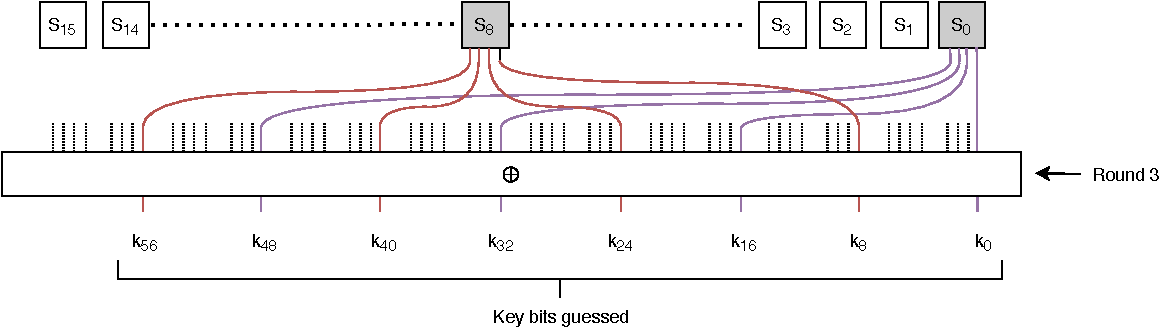
\includegraphics[width=\linewidth]{DC2.pdf}
	\endminipage
	\caption{Guess 8 bits of the key $k_2$}
	\label{fig:dc2}
\end{figure}\\
We are able to find 8 bits of key $k_2$. In our case only  8 bit right  subkey holds for all $2^{14}$ filtered pairs or in other word highest counter indicate the right 8 bit subkey.
\end{frame}

\begin{frame}{Complexity Analysis}
    \begin{block}{Complexity}
    \textbf{(Data, Time, Memory)} = $(2^{19},2^{25.17},2^{14})$
    \end{block}
\end{frame}

\section{Linear Cryptanalysis}

\begin{frame}{LAT of the S-box}
	\begin{figure}[h!]
	\centering
	\scalebox{0.8}{
		\begin{tabular}{ |c||c|c|c|c|c|c|c|c|c|c|c|c|c|c|c|c| }
			\hline
			& 0 & 1 & 2 & 3 & 4 & 5 & 6 & 7 & 8 & 9 & A & B & C & D & E & F  \\ \hline \hline
			0& 8 & - & - & - & - & - & - & - & - & - & - & - & - & - & - & - \\ 
			1& - & - & - & - & - & -4 & - & -4 & - & - & - & - & - & -4 & - & 4 \\
			2& - & - & 2 & 2 & -2 & -2 & - & - & 2 & -2 & - & 4 & - & 4 & -2 & 2 \\
			3& - & - & 2 & 2 & 2 & -2 & -4 & - & -2 & 2 & -4 & - & - & - & -2 & -2 \\
			4& - & - & -2 & 2 & -2 & -2 & - & 4 & -2 & -2 & - & -4 & - & - & -2 & 2 \\
			5 & - & - & -2 & 2 & -2 & 2 & - & - & 2 & 2 & -4 & - & 4 & - & 2 & 2\\
			6 & - & - & - & -4 & - & - & -4 & - & - & -4 & - & - & 4 & - & - & -\\
			7 & - & - & - & 4 & 4 & - & - & - & - & -4 & - & - & - & - & 4 & -\\
			8 & - & - & 2 & -2 & - & - & -2 & 2 & -2 & 2 & - & - & -2 & 2 & 4 & 4\\
			9 & - & 4 & -2 & -2 & - & - & 2 & -2 & -2 & -2 & -4 & - & -2 & 2 & - & -\\
			A & - & - & 4 & - & 2 & 2 & 2 & -2 & - & - & - & -4 & 2 & 2 & -2 & 2\\
			B & - & -4 & - & - & -2 & -2 & 2 & -2 & -4 & - & - & - & 2 & 2 & 2 & -2\\
			C & - & - & - & - & -2 & -2 & -2 & -2 & 4 & - & - & -4 & -2 & 2 & 2 & -2\\
			D & - & 4 & 4 & - & -2 & -2 & 2 & 2 & - & - & - & - & 2 & -2 & 2 & -2\\
			E & - & - & 2 & 2 & -4 & 4 & -2 & -2 & -2 & -2 & - & - & -2 & -2 & - & -\\
			F & - & 4 & -2 & 2 & - & - & -2 & -2 & -2 & 2 & 4 & - & 2 & 2 & - & -\\
			\hline
	\end{tabular}}
\captionof{table}{Linear Approximation Table}
\end{figure}
\end{frame}

\begin{frame}{Observations}
\begin{itemize}
	\item Maximum bias $\leq2^{-2}$
	\item For a Single bit $\leq2^{-3}$
	\item Bias Computation \begin{equation*}
		2^{m-1}\prod_{i=1}^{m} \epsilon_i
	\end{equation*}
\end{itemize}
\end{frame}

\begin{frame}{Analysis}
\begin{itemize}
	\item Total 3 Cases to analyse the linear approximation of 4 rounds
	\item Results to bound the linear approximation bias for 28 rounds
	\item Let $\epsilon_{4R}$ be the maximal bias of a linear approximation of four
	rounds of present, then $\epsilon_{4R}\leq\frac{1}{2^7}$
\end{itemize}
\end{frame}

\begin{frame}{Proof$\ldots$}
	\begin{itemize}
		\item Bias Calculation for 4 S-boxes:
		\begin{equation*}
			\epsilon_4^{4} \leq 2^{4-1} \times (2^{-2})^2 \times (2^{-3})^2 \implies \epsilon_4^{4} \leq 2^{-7}
		\end{equation*}
		\item Bias Calculation for 5 S-boxes:
	    \begin{equation*}
	    	\epsilon_4^{5} \leq 2^{5-1} \times (2^{-2})^4 \times (2^{-3}) \implies \epsilon_4^{5} \leq 2^{-7}
	    \end{equation*}
	\end{itemize}
\end{frame}

\begin{frame}{Resistent to the Linear Attack}
	\begin{itemize}
		\item Maximal Bias for 28-round linear approximation
		\item Now assume that the cryptanalyst needs to approximate only only 28 rounds
		\item So total $2^{86}$ known plaintexts are required 
		\item Which are greater than the available plaintexts space, that is $2^{64}$
		\item Proved
	\end{itemize}
\end{frame}
\section{Integral property}

\begin{frame}{5-round integral distinguishers for PRESENT}
Input:\\(ccccccccccccccccccccccccccccccccccccccccccccccccccccccccccccaaaa)\\
Output:\\(????????????????????????????????????????????????????????bbbb)\\\\
c: constant bit, a: active bit, b: balanced bit, ?: unknown bit\\
\begin{block}{Note}
     In this experiment, we are taking $2^{12}$ messages and varying right most 4 bits.
\end{block}
\end{frame}
\section{Brownie Point Nominations}

\begin{frame}{Brownie Point}
   \begin{block}{}
   \begin{enumerate}
    	\item Using the idea of differential and filtering taught in the course, we have implemented a differential attack on 3 Rounds of PRESENT. 
     	\item We have verified 5 Rounds integral property of PRESENT.
   \end{enumerate}
      \end{block}
\end{frame}


\section{Conclusion}

\begin{frame}{Conclusion}
   \begin{itemize}
    \item Understanding the design choices of PRESENT cipher. 
    \item Properties of S-box
    \item Resistance against cryptographic attacks
    \item Implementation of 3-Rounds differential attack
    \item verify 5 round integral property 
    \item Linear Cryptanalysis
\end{itemize}

\end{frame}



\begin{frame}{Thanks}
\begin{block}{Team Members}
	\begin{itemize}
	    \item Ajay Tarole
		\item Ashish Kumar Suraj
		\item Rudraksh Kashyap
	\end{itemize}
\end{block}
\begin{block}{Implementation Info}
	\begin{itemize}
		\item Github Link: \href{https://github.com/ajay0090/PRESENT-Cipher}{https://github.com/ajay0090/PRESENT-Cipher}
	\end{itemize}
\end{block}
\end{frame}
\end{document}
